\date{\today}
\title{Assignment 4: CS 763, Computer Vision}
\author{Sasank Chilamkurthy\\ Tharun Kumar Reddy\\ Rajeev Puppala}

\documentclass[11pt]{article}

\usepackage{amsmath}
\usepackage{amssymb}
%\usepackage{hyperref}
%\usepackage{ulem}
\usepackage{graphicx}
\usepackage[margin=0.5in]{geometry}
\begin{document}
\maketitle


\begin{enumerate}
\item Answer the following questions pertaining to the essential/fundamental matrix in a binocular stereo system:
\begin{enumerate}
\item Consider two cameras with parallel optical axes, with the optical center of the second camera at a location $(a,0,0)$ as measured in the first camera's coordinate frame. What is the essential matrix of this stereo system? \\
Ans. Rotation matrix is Identity Matrix since the axis are parallel and $\textbf{T} = (a,0,0)$ \\
$\implies \textbf{T}_x = a; \textbf{T}_y = 0; \textbf{T}_z = 0$\\
$\implies \textbf{S} = \begin{bmatrix}
0 &0 &0\\
0 &0 &-a\\
0 &a &0\\
\end{bmatrix}$\\
Therefore $\textbf{E} = \textbf{R}\textbf{S}$\\
$\implies \textbf{E} = \begin{bmatrix}
0 &0 &0\\
0 &0 &-a\\
0 &a &0\\
\end{bmatrix}$
\item Suppose I gave you the fundamental matrix of a stereo system, how will you infer the left and right epipoles?\\
Ans.  The left epipole lies on all epipolar lines in the
left image. Hence we can write\\
$\tilde{P_r^t}\textbf{F}\tilde{e_l} = 0$\\
$\therefore \textbf{F}\tilde{e_l} =0$
$\implies \tilde{e_l}$ lies in the nullspace of $\textbf{F}$\\
In the same way $\tilde{e_r}$ is the nullspace of $\textbf{F}^T$\\
When $\textbf{F}$ is written as $ \textbf{U}_\textbf{F}\textbf{S}_\textbf{F}\textbf{V}_\textbf{F}^T$\\
$\tilde{e_l}$ is column of $\textbf{V}_\textbf{F}$ corresponding to null singular value\\ 
$\tilde{e_r}$ is column of $\textbf{U}_\textbf{F}$ corresponding to null singular value
\item Prove that any essential matrix will have one singular value which is zero, and that its other two singular values are identical. Derive a relationship between these singular values and the extrinsic parameters of the stereo system (\textit{i.e.}, the rotation matrix $\textbf{R}$ and/or the translation vector $\textbf{t}$ between the coordinate frames of the two cameras). [Hint: Show that if $\textbf{E}$ is the essential matrix, then we can write $\textbf{E}^T \textbf{E} = \alpha (\textbf{I}_{3 \times 3} - \textbf{t}_\textbf{u} \textbf{t}^T_\textbf{u})$ where $\alpha$ is some scalar which you should express in terms of $\textbf{R}$ and/or $\textbf{t}$, $\textbf{I}_{3 \times 3}$  is the identity matrix with 3 rows and 3 columns, and $\textbf{t}_\textbf{u}$ is a vector of unit magnitude in the direction of $\textbf{t}$]. \\
Ans. $\textbf{E}^T \textbf{E} = (\textbf{R}\textbf{S})^T(\textbf{R}\textbf{S}) = \textbf{S}^T\textbf{R}^T\textbf{R}\textbf{S} = \textbf{S}^T\textbf{S}$\\
$\textbf{S} = \begin{bmatrix}
0 &-T_z &T_y\\
T_z &0 &-T_x\\
-T_y &T_x &0\\
\end{bmatrix}$\\
$\implies \textbf{S}^T\textbf{S} = \begin{bmatrix}
T_z^2+T_y^2 &-T_yT_x &-T_xT_z\\
-T_yT_x &T_z^2+T_x^2 &-T_yT_z\\
-T_xT_z &-T_yT_z &T_x^2+T_y^2\\
\end{bmatrix} = (T_x^2+T_y^2+T_z^2)(\textbf{I}_{3 \times 3} - \textbf{t}_\textbf{u} \textbf{t}^T_\textbf{u})$ \\where $\textbf{t}_\textbf{u} = \begin{pmatrix}
\frac{T_x}{\sqrt{T_x^2+T_y^2+T_z^2}}\\
\frac{T_y}{\sqrt{T_x^2+T_y^2+T_z^2}}\\
\frac{T_z}{\sqrt{T_x^2+T_y^2+T_z^2}}\\
\end{pmatrix} $is a vector of unit magnitude in the direction of $\textbf{t}$\\
Let $v$ be an eigen vector of $\textbf{E}^T \textbf{E}$ and $\lambda$ be its eigen value.
$v$ can be written as $\lambda_1\textbf{t}_\textbf{u}+\lambda_2\textbf{t}_{\textbf{u}\perp}$\\
where $\textbf{t}_{\textbf{u}\perp}$ is an unit magnitude perpendicular vector to 
$\textbf{t}_\textbf{u}$ and $\lambda_1$ and $\lambda_2$ are the corresponding dot products of $v$ with $\textbf{t}_\textbf{u}$ and $\textbf{t}_{\textbf{u}\perp}$.\\
Substituting $v$ in the above equation gives\\
 $\alpha (\textbf{I}_{3 \times 3} - \textbf{t}_\textbf{u} \textbf{t}^T_\textbf{u}) v = \lambda v$ where $\alpha = T_x^2+T_y^2+T_z^2$\\
 $\implies (\alpha - \lambda)(\lambda_1\textbf{t}_\textbf{u} + \lambda_2\textbf{t}_{\textbf{u}\perp}) = \alpha\textbf{t}_\textbf{u}\textbf{t}_\textbf{u}^T(\lambda_1\textbf{t}_\textbf{u} + \lambda_2\textbf{t}_{\textbf{u}\perp})$\\
 $\implies (\alpha - \lambda)\lambda_1\textbf{t}_\textbf{u} + (\alpha - \lambda)\lambda_2\textbf{t}_{\textbf{u}\perp} = \alpha\lambda_1\textbf{t}_\textbf{u} + 0$ \\
 $\implies \lambda\lambda_1 = 0$ and $(\alpha - \lambda)\lambda_2 = 0$\\
 Therfore as both $\lambda_1$ and $\lambda_2$ cannot be simultaneously $0$ \\
 if $\lambda_1 = 0$ then $\alpha = \lambda$ and \\
 if $\lambda_2 = 0$ then $\lambda = 0$\\
 In the first case we can find two vectors that are not parallel to each other and perpendicular to $\textbf{t}_\textbf{u}$\\
 $\therefore$ one eigen value is $0$ and other two eigen values are same and equal to $\alpha$\\
Singular values of essential matrix are square roots of eigen values of $\textbf{E}^T \textbf{E}$\\
$\therefore$ singular values of $\textbf{E}$ are $0,\sqrt{T_x^2+T_y^2+T_z^2},\sqrt{T_x^2+T_y^2+T_z^2}$.
\item In the noiseless case, what is the minimum number of corresponding pairs of points you must know in order to estimate the essential matrix? Or in other words, how many degrees of freedom does an essential matrix have? Justify your answer. (Think carefully). \\
Ans. $\textbf{E} = \textbf{R}\textbf{S}$\\
$\textbf{R}$ is rotation matrix. $\therefore$ DOF of $\textbf{R} = 3$\\
$\textbf{S}$ is Transition matrix. $\therefore$ DOF of $\textbf{S} = 3$\\
$\implies$ DOF of $\textbf{E}$ should be $6$ But if $\textbf{E}$ is an essential matrix then $\alpha\textbf{E}$ can also be an essential matrix  for any scalar $\alpha$ for the same system \\
Therefore by fixing $\alpha$ we can reduce the DOF of $\textbf{E}$ by $1$\\
$\therefore$ Degrees of freedom for essential matrix $\textbf{E} = 5$\\
$\implies 5$ pairs of corresponding pairs of points are required to estimate essential matrix
\item We have studied the eight-point algorithm in class for estimating the essential/fundamental matrix. There exist algorithms that require only 7 pairs of corresponding points. In robust estimation, what main advantage will a 7-point algorithm have over the 8-point version? \\
Ans. In robust estimation using RANSAC method the no. of sets of pairs of corresponding points points to be taken to maximise the probability of finding  a set with all inliers is less if we use $7-$point algorithms instead of $8-$point algorithm for a given precentage of outliers $(p)$
\end{enumerate}
\textsf{[1 + 1 + 5 + 1 + 2 = 10 points]}

\item In class, we have seen (or will soon see) a method of normalizing matching points from the two given images, before computing the fundamental matrix or the homography transformation (you would have seen this normalization in the code for homography that was handed out in assignment 2). This normalization involves zero-centering each individual point-set followed by a rescaling. Express this normalization in the form of a matrix, and write out the expression for the final fundamental matrix. Explain why this normalization is useful. \textsf{[5 points]}.\\
Ans. The origin of the new coordinate system should be centered at the centroid of the image points. This is accomplished by a translation of the original origin to the new one and after the translation the coordinates are uniformly scaled so that the mean distance from the origin to a point equals  $\sqrt{2}$.\\
The final transformation matrix will be a product of  a scalar and transition matrix which will normalize the image coordinates.\\
New homogeneous image coordinates  $\mathbf{\bar y}, \mathbf{\bar y}'$  are given by\\
 $\mathbf{\bar y} = \mathbf{T} \, \mathbf{y}\\ 
 \mathbf{\bar y}' = \mathbf{T}' \, \mathbf{y}'$ \\
 where  $\mathbf{T}, \mathbf{T}'$  are the transformations of the two images from the old to the new normalized image coordinates.\\
 Epipolar constraint based on the fundamental matrix can now be rewritten as\\
$(\mathbf{\bar y}')^{T} \, ((\mathbf{T}')^{T})^{-1} \, \mathbf{F} \, \mathbf{T}^{-1}\, \mathbf{\bar y} = (\mathbf{\bar y}')^{T} \, \mathbf{\bar F} \, \mathbf{\bar y} = 0$\\
$\implies \mathbf{\bar F} = ((\mathbf{T}')^{T})^{-1} \, \mathbf{F} \, \mathbf{T}^{-1}$ where $\mathbf{\bar F}$ is the new fundamental matrix for normalised coordinates.\\
The de-normalised fundamental matrix is given by\\
$ \mathbf{F} = (\mathbf{T}')^{T} \, \mathbf{\bar F} \, \mathbf{T} $\\
This Normalisation reduces the problem caused by the poor distribution of the homogeneous image coordinates in their space.
\item In this exercise, you will implement the Adaboost method for creating a strong binary classifier from a series of weaker classifiers. You will work with some synthetic datasets and also with a dataset containing images of digits.
\\
Consider a training set consisting of $N$ input vectors $\{\textbf{x}_j\}_{j=1}^{N}$ in a $d$-dimensional space, and their respective labels $\{y_j\}_{j=1}^N$ where $\forall j, y_j \in \{-1,+1\}$. You will assign a scalar weight to each input vector. Before the first iteration of Adaboost, these weights will be set to be equal in value. In each round $t$, you will pick the best classifier from the following family of weak classifiers: $h_t(\textbf{x}; i,p,\theta) = \textrm{sign}(p(x_i - \theta))$ where $x_i$ is the $i^{\textrm{th}}$ element of $d$-dimensional input vector $\textbf{x}$, the parameter $p \in \{-1,+1\}$ and $\theta$ is a real-valued threshold parameter. Basically, this classifier assigns input vector $\textbf{x}$ the label `+1' if either (1) $x_i > \theta$ and $p = +1$, or (2) $x_i \leq \theta$ and $p=-1$. Otherwise it assigns $\textbf{x}$ the label `-1'. The best classifier refers to the classifier producing the least weighted error on the training set, i.e. least value of $\epsilon = \sum_{j=1}^N w_j I(h_t(\textbf{x}_j) \neq y_j)$ where $I(.)$ is an indicator function that returns 1 if the predicate passed as a parameter is true, and returns 0 otherwise. Note that the search for the best classifiers involves picking the tuple $(i,p,\theta)$. After picking the best classifier, you will update the weights following the method in the standard Adaboost algorithm. This entire process is repeated for $T$ rounds. You need to specify the value of $T$ but $T = 30$ to $40$ is sufficient. The final classifier after $T$ rounds will have the form $H(\textbf{x}) = \textrm{sign}(\sum_{t=1}^{T} \alpha_t h_t(\textbf{x}))$. 
\\
You will work with the following datasets. 
\begin{enumerate}
\item A dataset containing 2000 points in 2D drawn from a [0,1] bounded uniform random distribution. Label all the points lying on or inside a rectangle bounded by the lines $x = 0.3$, $x = 0.7$, $y = 0.3$, $y= 0.7$ as $+1$ and the rest as $-1$. Randomly divide this dataset into disjoint sets of 1000 training points and 1000 test points (called dataset1). 

\item A dataset containing 2000 points in 2D drawn from a [0,1] bounded uniform random distribution. Label all the points satisfying any of the following conditions as `+1' and the rest as `-1': (1) lying on or inside a rectangle bounded by the lines $x = 0.3$, $x = 0.7$, $y = 0.3$, $y= 0.7$ as $+1$ , (2) with x-coordinate between 0.15 and 0.25 or between 0.75 and 0.85, (3) with y-coordinate between 0.15 and 0.25 or between 0.75 and 0.85. Randomly divide this dataset into disjoint sets of 1000 training points and 1000 test points (called dataset2). 

\item A dataset containing 2000 points in 2D drawn from a zero-mean Gaussian distribution of standard deviation 2. Label all the points whose distance from the origin is less than 2 as +1 and the rest as -1. Randomly divide this dataset into disjoint sets of 1000 training points and 1000 test points (called dataset3). 



\item A dataset containing 2000 points in 2D drawn from a zero-mean Gaussian distribution of standard deviation 2. Label all the points whose distance from the origin is either less than 2, or between 2.5 and 3, as +1 and the rest as -1. Randomly divide this dataset into disjoint sets of 1000 training points and 1000 test points (called dataset4). 


\item The text files can be read into MATLAB using `dlmread'. Each image has size $13 \times 13$, and there are 1000 images each in the training set as well as the test set. Label the images belonging to any one digit (say `2' or `3') as `+1' and all the others as `-1'. Thus for this database, your job is to determine whether a given image contains the selected digit or not.


\end{enumerate}
For each of the five datasets, do the following after each round of Adaboost: (1) estimate and print the training error of the \emph{strong} classifier created thus far, (2) estimate and print the error of the \emph{strong} classifier created thus far on the \emph{test} set. For the first four datasets, also plot the test points with their associated labels using the MATLAB function called `scatter' (in each round of Adaboost). Sample scatter plots for the first four datasets can be found at (named as dataset1.jpg and so on). Finally, for all four datasets, plot a graph of the test set error versus the number of rounds of Adaboost. Do you notice something peculiar with the fourth dataset? Explain what you would you do to remedy that situation (there is no need to implement). 
\end{enumerate}
\textsf{[15 points]}
\begin{itemize}
	\item In part d, error rate is unusually high. This is because concentric circular boundaries are hard to capture with classifiers of the form $\textrm{sign}(p(x_i - \theta))$. So, this problem can be solved by including classifiers of the form $\textrm{sign}(p(r - \phi))$ where $r$ is distance from the origin.
		\begin{figure}[h]
			\centering
			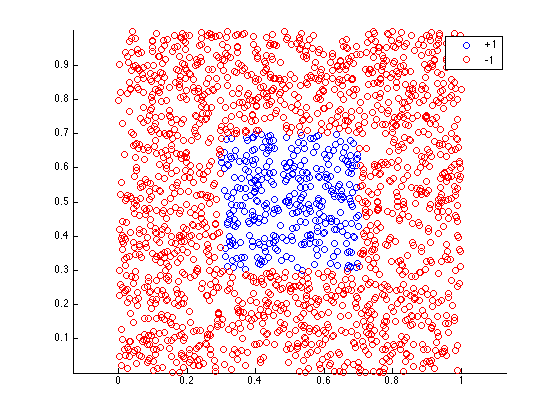
\includegraphics[width=3.5in]{part_a_scatter.png}
			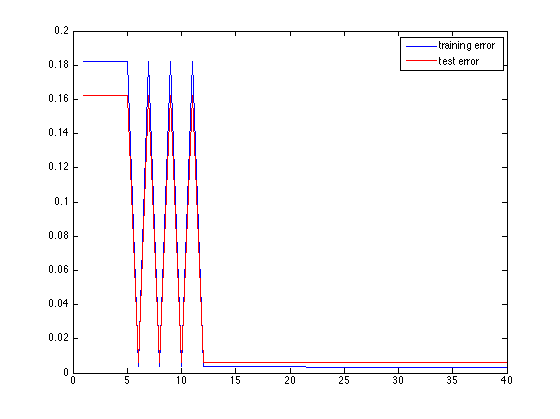
\includegraphics[width=3.5in]{part_a.png}
			\caption{Part a}
		\end{figure}
		
		\begin{figure}[h]
			\centering
			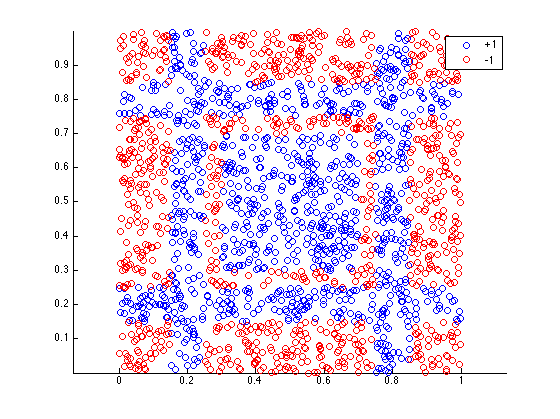
\includegraphics[width=3.5in]{part_b_scatter.png}
			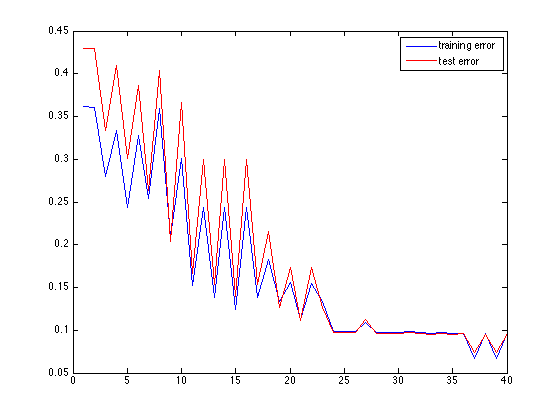
\includegraphics[width=3.5in]{part_b.png}
			\caption{Part b}
		\end{figure}
		
		\begin{figure}[h]
			\centering
			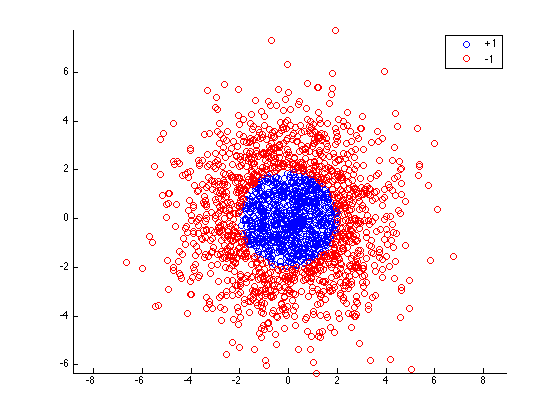
\includegraphics[width=3.5in]{part_c_scatter.png}
			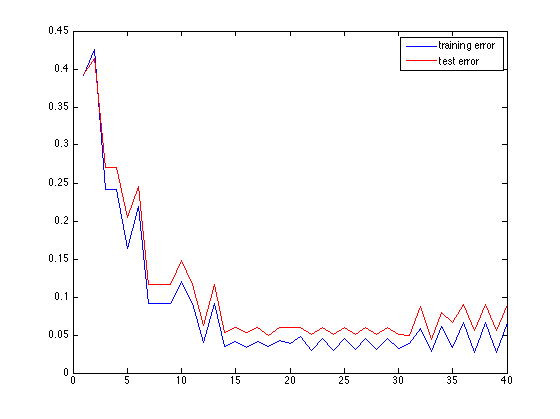
\includegraphics[width=3.5in]{part_c.png}
			\caption{Part c}
		\end{figure}
		
		\begin{figure}[h]
			\centering
			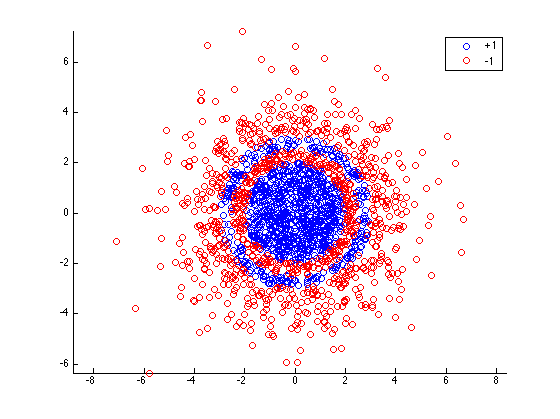
\includegraphics[width=3.5in]{part_d_scatter.png}
			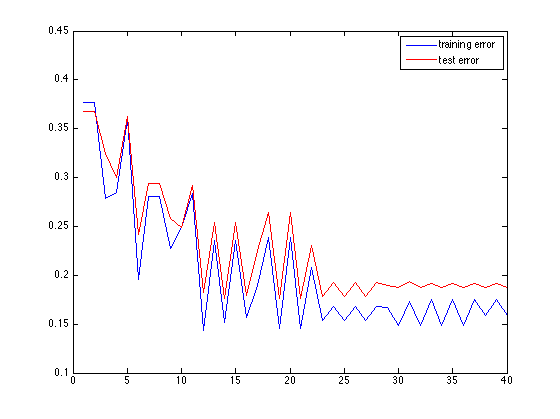
\includegraphics[width=3.5in]{part_d.png}
			\caption{Part d}
		\end{figure}
	
		\begin{figure}[h]
			\centering
			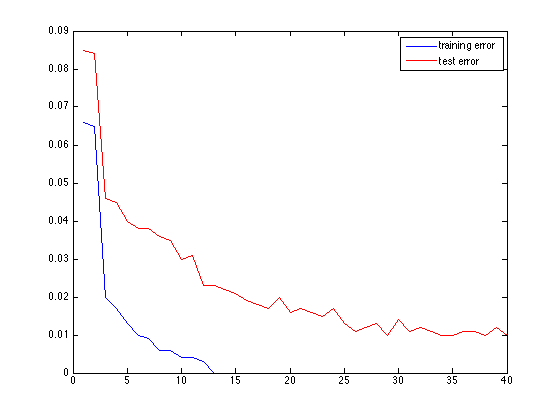
\includegraphics[width=3.5in]{part_e.png}
			\caption{Part e}
		\end{figure}

\end{itemize}


\end{document}